\label{chap:ExpRes}
Based on sections \ref{sec:neuralNet} and \ref{sec:imgClass}, in this chapter, we will discuss further about the experimental results, particularly of the image classification, distance estimation and object detection problems.

\section{Image Classification}
\subsection{Problem Review}
Remind that the problem we are referring in this section is the image classification of images belonging to 12 categories. We have the following details:
\begin{enumerate}
	\item 12 classes: \tit{"apple", "pen", "book", "monitor", "mouse", "wallet", "keyboard", "banana", "key", "mug", "pear", "orange"}.
	\item 1200 images for each class.
	\item Divide the whole dataset into 30\% test set (4320 images), 56\% training set (8064 images) and 14\% validation set (2016 images).
	\item Experiments with multiple options: 
	\begin{itemize}
		\item with/without fine-tuning
		\item with/without image preprocessing
		\item with/without data augmentation
		\item multiple based models (Resnet50, VGG16, Xception)
		\item multiple configuration for fully-connected layer (number of hidden layer, etc.)
	\end{itemize} 
	\item Note that after convolutional block, we flatten the feature tensor to become a 1D feature vector. In addition, our number of classes is fixed to 12. Hence we only denote the hidden layers in the fully-connected part. For example, resnet\_512 is the model uses convolutional blocks of Resnet50 and has fully-connected part as: flatten - 512 - 12. 
\end{enumerate}

\subsection{Transfer Learning Result}
%\subsection{Results and Observations}
As discussed in subsection \ref{sec:transferLearning}, we can freely design the fully-connected part. After multiple experiments, I found the following interesting observations:
\begin{enumerate}
	\item Bigger fully-connected parts only helps to train the system in fewer epochs. This is reasonable because more complex models has more capacity. However, the trade-off is that we have a bigger model size and it is slower at test time. (figure \ref{fig:compareResnetNoFT})
	\item Fine-tuning the final convolutional block improves the accuracy about 2-3\% (figure \ref{fig:accResnet128NoFT} vs figure \ref{fig:accResnet128})
	\item Image augmentation do not help much in my situation (\ref{fig:compareResnet}). We can see that models with augmented data have better performance in the beginning. However at the end, they are all rougly the same.
	\item As expected, zero-centering and normalization improves a bit the training accuracy (i.e. faster training) but does not improve significantly the validation accuracy. (figures \ref{fig:resnet512StMean}, \ref{fig:accResnet512}, \ref{fig:resnet512StMeanScale}, \ref{fig:accResnet512dup}) I think the reason that it does not improve validation accuracy significantly is the difficulty of our dataset.
	\item Resnet50 is the best base model among VGG16, Xception and Resnet50 (more details are shown in figure \ref{fig:compareModels}). A more carefully fine-tuned version of resnet\_512 model can reach to 94.2\% on validation accuracy.
	\item Accuracy on test set is $\approx$ 93.5\% - 93.7\%. Prediction details can be found in table \ref{table:1}. 
	\item Remark that our dataset is difficult because:
	\begin{itemize}
		\item one image can contain objects of several classes belonging to the 12 categories
		\item the ground truth object does not necessarily appear largely at the center of the image
	\end{itemize}
	Figure \ref{fig:testFail1} and \ref{fig:testFail2} illustrate 2 examples where the system predicts wrongly.
\end{enumerate}
	

\begin{figure}[tb]
	\centering
	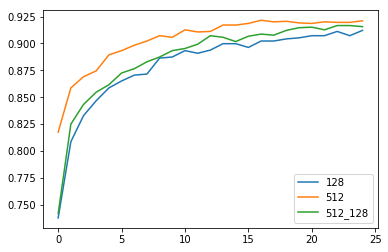
\includegraphics[width=0.6\hsize]{./figures/compareResnetNoFT}
	\caption{Comparison of Resnet models with different fully-connected parts: 128, 512, 512\_128. We can see that bigger model (512) has more capacity and reach the baseline 90\% faster. Multiple layers (512\_128) on the other hand performs worse than one big layer (512).}
	\label{fig:compareResnetNoFT}
\end{figure}

\begin{figure}[!ht]
	\centering
	\begin{minipage}[t]{0.45\linewidth}
		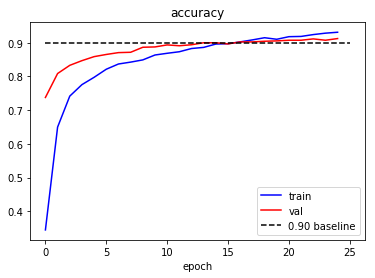
\includegraphics[scale=0.5]{./figures/accResnet128NoFT}
		\caption{resnet\_128 without finetuning: validation accuracy reaches to  $\approx$ 91.6\%}
		\label{fig:accResnet128NoFT}
	\end{minipage}
	\centering
	\begin{minipage}[t]{0.45\linewidth}
		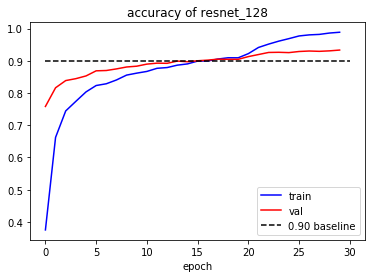
\includegraphics[scale=0.5]{./figures/accResnet128}
		\caption{resnet\_128 fine-tuned around epoch 18: validation accuracy reaches to $\approx$ 93.3\%}
		\label{fig:accResnet128}
	\end{minipage}
\end{figure}


\begin{figure}[tb]
	\centering
	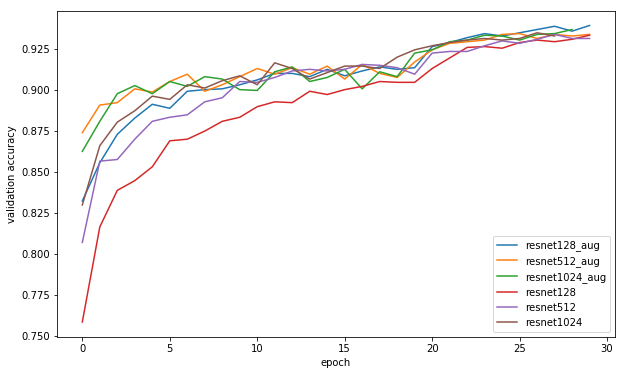
\includegraphics[width=0.8\hsize]{./figures/compareResnet}
	\caption{Comparison of Resnet models with different fully-connected parts: 128, 512, 1024 and with/without data augmentation. We can see that augmentation data does not help much in the end. In the beginning, the accuracy when applying data augmentation is higher because the system is trained on the augmented images (i.e. more training data). Note that all models jumped up around epoch 20 when I applied fine-tuning.}
	\label{fig:compareResnet}
\end{figure}


\begin{figure}[!ht]
	\centering
	\begin{minipage}[t]{0.45\linewidth}
		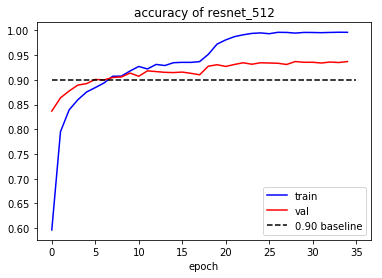
\includegraphics[scale=0.5]{./figures/resnet512StMean}
		\caption{resnet\_512 with mean of training data subtracted. Train accuracy is a bit higher at the beginning.}
		\label{fig:resnet512StMean}
	\end{minipage}
	\centering
	\begin{minipage}[t]{0.45\linewidth}
		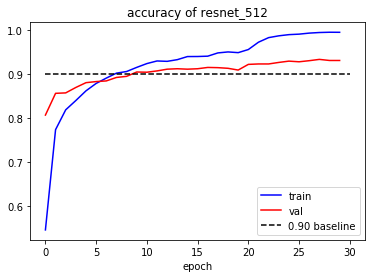
\includegraphics[scale=0.5]{./figures/accResnet512}
		\caption{resnet\_512 with no preprocessing. Both two versions reach $\approx 93.7\%$ validation accuracy at the end.}
		\label{fig:accResnet512}
	\end{minipage}
\end{figure}

\begin{figure}[!ht]
	\centering
	\begin{minipage}[t]{0.45\linewidth}
		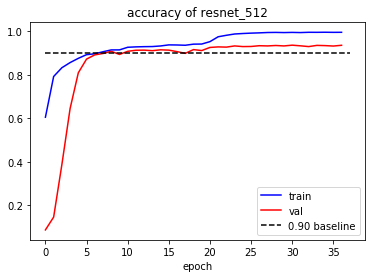
\includegraphics[scale=0.5]{./figures/resnet512StMeanScale}
		\caption{resnet\_512 with both mean of training data subtracted and scaled by dividing to 255. Training is a bit faster but validation accuracy is improving more slowly.}
		\label{fig:resnet512StMeanScale}
	\end{minipage}
	\centering
	\begin{minipage}[t]{0.45\linewidth}
		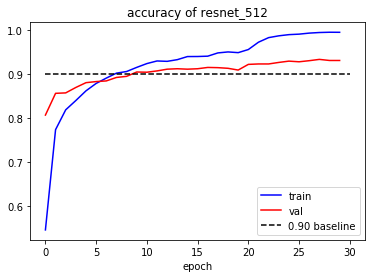
\includegraphics[scale=0.5]{./figures/accResnet512}
		\caption{resnet\_512 with no preprocessing. Both two versions reach $\approx 93.7\%$ validation accuracy at the end.}
		\label{fig:accResnet512dup}
	\end{minipage}
\end{figure}


\begin{figure}[tb]
	\centering
	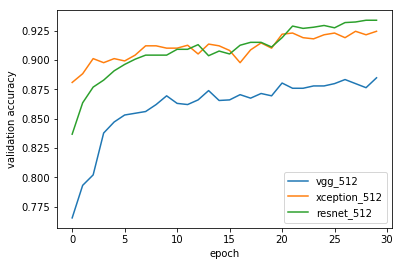
\includegraphics[width=0.7\hsize]{./figures/compareModels}
	\caption{Comparison accross models: VGG16, Resnet50, Xception with the same fully-connected layer (512). We see clearly the model capacity affects the result: VGG16 can not reach base-line 90\% while advanced models like Resnet50 and Xception easily get over 92\%. More precisely, Resnet50 is the best with accuracy greater than $93\%$) and Xception's accuracy is around $92.5\%$.}
	\label{fig:compareModels}
\end{figure}

\begin{figure}[tb]
	\centering
	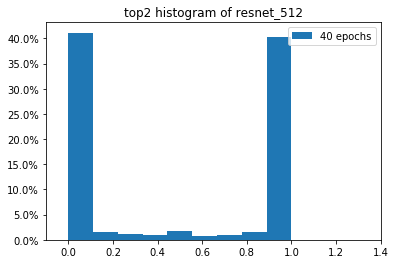
\includegraphics[width=0.6\hsize]{./figures/top2Histo}
	\caption{Histogram of Top 2 predictions probability on test set after training. As expected the trained model is quite sure about its predictions (mostly in $>0.9$ for the maximal probability and $<0.1$ for the second maximal probability). Some samples in the middle represents well the case it is confused due to the difficulty of the dataset.}
	\label{fig:top2Histo}
\end{figure}

\begin{table}[h!]
	\centering
\scriptsize		
	\begin{tabular}{ |c|c|c|c|c|c|c|c|c|c|c|c|c| } 
		\hline
 class &  apple &  pen &  book &  monitor &  mouse &  wallet &  keyboard &  banana &  key &  mug &  pear &  orange \\
 \hline
 apple &  \tbf{0.83} &  0.00 &  0.01 &  0.00 &  0.01 &  0.00 &  0.00 &  0.03 &  0.00 &  0.00 &  0.05 &  0.07 \\
 \hline
 pen &  0.00 &  \tbf{0.96} &  0.00 &  0.00 &  0.01 &  0.01 &  0.00 &  0.00 &  0.01 &  0.00 &  0.00 &  0.00 \\
 \hline
 book &  0.00 &  0.01 &  \tbf{0.96} &  0.01 &  0.00 &  0.02 &  0.00 &  0.00 &  0.00 &  0.00 &  0.00 &  0.00 \\
 \hline
 monitor &  0.00 &  0.01 &  0.01 &  \tbf{0.94} &  0.02 &  0.01 &  0.01 &  0.00 &  0.00 &  0.00 &  0.00 &  0.00 \\
 \hline
 mouse &  0.01 &  0.00 &  0.00 &  0.03 &  \tbf{0.88} &  0.01 &  0.04 &  0.00 &  0.01 &  0.01 &  0.01 &  0.00 \\
 \hline
 wallet &  0.00 &  0.00 &  0.01 &  0.01 &  0.00 &  \tbf{0.96} &  0.00 &  0.00 &  0.02 &  0.00 &  0.00 &  0.00 \\
 \hline
 keyboard &  0.00 &  0.00 &  0.00 &  0.04 &  0.02 &  0.00 &  \tbf{0.94} &  0.00 &  0.00 &  0.00 &  0.00 &  0.00 \\
 \hline
 banana &  0.02 &  0.00 &  0.00 &  0.00 &  0.00 &  0.00 &  0.00 &  \tbf{0.95} &  0.00 &  0.00 &  0.00 &  0.03 \\
 \hline
 key &  0.00 &  0.00 &  0.01 &  0.00 &  0.00 &  0.01 &  0.00 &  0.00 &  \tbf{0.97} &  0.00 &  0.00 &  0.00 \\
 \hline
 mug &  0.00 &  0.00 &  0.00 &  0.00 &  0.00 &  0.00 &  0.00 &  0.01 &  0.00 &  \tbf{0.99} &  0.00 &  0.00 \\
 \hline
 pear &  0.05 &  0.00 &  0.00 &  0.00 &  0.00 &  0.00 &  0.00 &  0.01 &  0.00 &  0.00 &  \tbf{0.91} &  0.02 \\
 \hline
 orange &  0.03 &  0.00 &  0.00 &  0.00 &  0.00 &  0.00 &  0.00 &  0.02 &  0.00 &  0.00 &  0.03 &  \tbf{0.92} \\
 \hline
	\end{tabular}
\caption{Prediction table: each row represents percentage of the system's predictions on the corresponding class. Consider the first row for example: for all images of ground truth \tit{apple}, the systems predicts correctly 83\%, 17\% wrong predictions false mostly to \tit{orange}, \tit{pear}. This is acceptable as noted previously that many fruit images contain objects of mixed classes.}
\label{table:1}
\end{table}

\begin{figure}[!ht]
	\centering
	\begin{minipage}[t]{0.45\linewidth}
		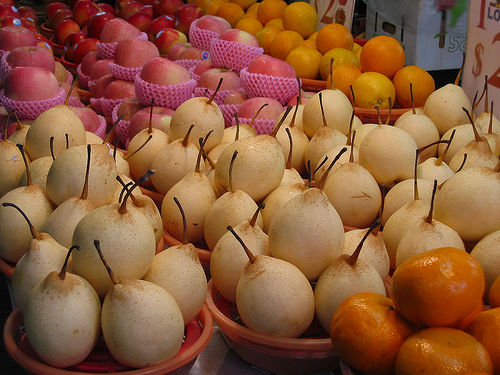
\includegraphics[scale=0.35]{./figures/testFail1}
		\caption{Model predicts \tit{orange} while ground truth is \tit{pear}. We can see that oranges appear in lower right corner and this type of pear is quite special.}
		\label{fig:testFail1}
	\end{minipage}
	\quad
	\begin{minipage}[t]{0.45\linewidth}
		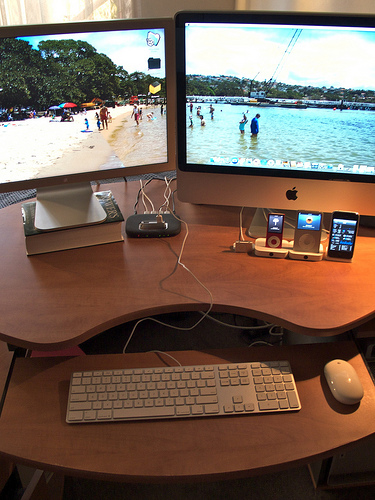
\includegraphics[scale=0.45]{./figures/testFail2}
		\caption{Model predicts \tit{monitor} while ground truth is \tit{keyboard}. We can see 2 bigs monitor in the upper of the image.}
		\label{fig:testFail2}
	\end{minipage}
\end{figure}

\section{Distance Estimation}
\label{sec:distEstimExp}
In this section, we set up an experiment to verify the distance estimation method described in section \ref{sec:camModel}. The experiment is done with the Cozmo robot facing straight ahead a cube. The cube size is 4.4cm (i.e $w = h = 4.4cm$). Remember that all camera parameters are presented in subsection \ref{subsec:camInfo}. The cube is placed at ground truth distance $z \in \{10, 20, 30, 40, 50\}$ (centimeters). Figure \ref{fig:distEstim} illustrates this point. 

\begin{figure}[tb]
	\centering
	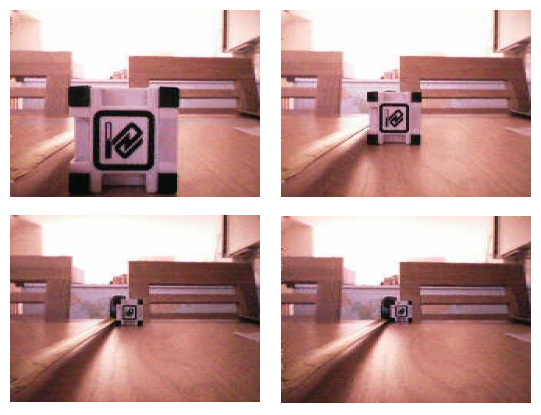
\includegraphics[width=0.6\hsize]{./figures/distEstim}
	\caption{Distance Estimation Experiment: a cube is placed in front of a Cozmo at distances $z = {10, 20, 40, 50}$ centimeters along the $z$ axis. We can see that there is no significant difference between $z = 40$ and $z = 50$ (centimeters). The size of the cube in the image are $w_i \approx {135, 70, 35, 28}$ (pixels) respectively.}
	\label{fig:distEstim}
\end{figure}

Explicitely, we will:
\begin{enumerate}
	\item compute $x_c, y_c, z$ from formula \ref{form:distEst} and \ref{form:centerIm}:
	\begin{align*}
	z = \frac{1}{2} (f_1 \frac{w}{w_i} + f_2 \frac{h}{h_i}) \hspace{0.5cm}
	x_c = \frac{1}{2}\frac{(u_1 + u_2 - 2  c_1)z}{f_1} \hspace{0.5cm} y_c = \frac{1}{2}\frac{(v_1 + v_2 - 2c_2)z}{f_2}
	\end{align*}
	\item compute distance $d$ and verify that $d \approx z$ ($z$ calculated above):
	$$d = \sqrt{x^2 + y^2 + z^2}$$
	\item estimate absolute error $\Delta z$ and relative error $\Delta z / z$ which is close to $\Delta d$ and $\Delta d / d$ respectively since $z \approx d$
\end{enumerate} 

By measuring the corners' coordinates, we obtain $u_1, u_2, v_1, v_2, w_i, h_i$ (in pixels). Knowing also $w = h = 4.4$ (centimeters) together with the camera parameters $f, c_1, c_2$ (in pixels), we can derive from the above formulas the following result:

\begin{table}[h!]
	\centering
	\begin{tabular}{c|c|c|c|c}
ground truth $z$ (cm) & $\hat{z}$ (cm) & $\hat{d}$ (cm) & $\Delta z$ (cm) & $\Delta z / z$ (\%)\\
\hline
10 & 9.34 & 9.43 & 0.57 & 5.7 \\
20 & 18.95 & 19.00 & 1.00 & 5.0 \\
30 & 28.32 & 28.35 & 1.65 & 5.5 \\
40 & 37.36 & 37.37 & 2.63 & 6.6  \\
50 & 46.02 & 46.04 & 3.96 & 7.9
	\end{tabular}
	\caption{Distance Estimation Result: }
	\label{table:2}
\end{table}

We can see from table \ref{table:2} that:
\begin{itemize} 
	\item $d \approx z$ and have an quantitative estimation about the errors.
	\item The relative error is already $6.5\%$ for this simple setup \tit{where no perspective view error, no bounding box error and no shape variance error are taken into account}. 
	\item In addition, the figures also show the limitation of the camera sensor: for every distance larger than 40 centimeters, we hardly see the cube (of size 4.4 centimeters) in the image (images in second row in figure \ref{fig:distEstim}). 
	\item In my opinion, the range to detect the cube (by a general detector, not accounting the tag on the cube) \tbf{is from 10 to 20 centimeters}. Therefore, a double-size object (of size 8.8 centimeters) are seen in 20 to 40 centimeters. This is quite limited to implement visual based simultaneous localization and mapping (SLAM) algorithm \cite{wiki:SLAM}. Remember that, the more recent Cozmo robots have a better camera sensor: VGA $640 \times 480$ resolution \cite{cozmoTech}. 
\end{itemize}

Based on these observations, implementing a visual-based SLAM system is more reasonably a future work when we have a more recent Cozmo.

\section{Object Detection}

TODO: 